\documentclass[border=6pt]{standalone}
\usepackage{tikz}
\usepackage{pgfplots}
\pgfplotsset{compat=1.18}
\usetikzlibrary{arrows.meta,positioning,shapes.geometric,fit,backgrounds,calc,decorations.pathreplacing,patterns,pgfplots.groupplots}
\tikzset{
  blk/.style={rectangle, rounded corners=2pt, draw=black!70, thick, fill=blue!6,
              minimum height=8mm, minimum width=20mm, align=center, font=\small},
  io/.style={rectangle, rounded corners=6pt, draw=black!70, thick, fill=green!8,
             minimum height=8mm, align=center, font=\small},
  proc/.style={rectangle, draw=black!70, thick, fill=orange!10, minimum height=8mm,
               align=center, font=\small},
  dec/.style={diamond, aspect=2, draw=black!70, thick, fill=yellow!15, align=center, font=\footnotesize},
  warnbox/.style={rectangle, rounded corners=2pt, draw=red!60!black, thick, fill=red!7,
                  minimum height=8mm, align=center, font=\small},
  oklbox/.style={rectangle, rounded corners=2pt, draw=green!45!black, thick, fill=green!8,
                 minimum height=8mm, align=center, font=\small},
  ar/.style={-{Latex[length=2mm]}, thick},
  arl/.style={-{Latex[length=2mm]}, thick, dashed, draw=black!55},
  lbl/.style={font=\footnotesize\itshape, text=black!60},
}
\definecolor{good}{RGB}{34,139,34}
\definecolor{bad}{RGB}{178,34,34}
\definecolor{warn}{RGB}{218,165,32}
\definecolor{pesblue}{RGB}{0,45,98}
\definecolor{complete}{RGB}{30,125,79}
\definecolor{partial}{RGB}{176,106,0}
\definecolor{blocked}{RGB}{166,43,43}
\begin{document}
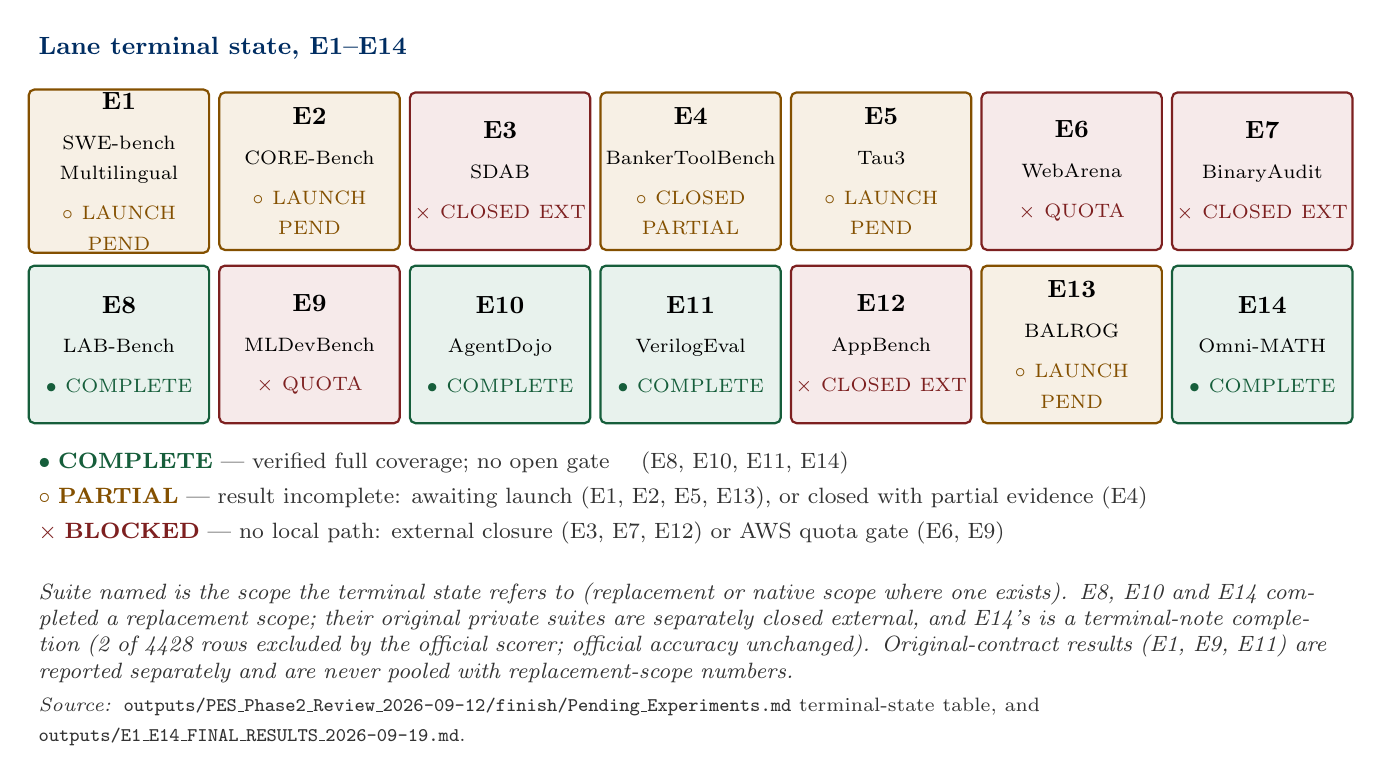
\begin{tikzpicture}[x=1mm,y=1mm,
  % one cell of the 14-lane status grid.
  % text width >= 22.2mm is required so the longest suite name
  % (BankerToolBench, 61.49pt at \scriptsize) sets on a single line.
  lcell/.style={rectangle, rounded corners=2pt, draw, thick, text width=22.2mm,
                minimum height=20mm, align=center, font=\small, inner sep=1pt},
  lcellC/.style={lcell, draw=complete!75!black, fill=complete!10},
  lcellP/.style={lcell, draw=partial!75!black,  fill=partial!10},
  lcellB/.style={lcell, draw=blocked!75!black,  fill=blocked!10},
  leg/.style={anchor=west, font=\footnotesize, text=black!80, align=left},
]

% grid left edge = cell centre (x=0) - half outer width ((22.2mm + 2pt)/2)
% = -11.45mm; heading, legend and footnotes align to it.

% ================= heading =================
\node[anchor=south west, font=\small\bfseries, text=pesblue] at (-11.45,13)
  {Lane terminal state, E1--E14};

% ================= row 1 : E1--E7 =================
\node[lcellP] at (0,0)
  {\textbf{E1}\\[1.2mm]{\scriptsize SWE-bench Multilingual}\\[1.2mm]{\scriptsize\textcolor{partial!75!black}{$\circ$\ LAUNCH PEND}}};
\node[lcellP] at (24.2,0)
  {\textbf{E2}\\[1.2mm]{\scriptsize CORE-Bench}\\[1.2mm]{\scriptsize\textcolor{partial!75!black}{$\circ$\ LAUNCH PEND}}};
\node[lcellB] at (48.4,0)
  {\textbf{E3}\\[1.2mm]{\scriptsize SDAB}\\[1.2mm]{\scriptsize\textcolor{blocked!75!black}{$\times$\ CLOSED EXT}}};
\node[lcellP] at (72.6,0)
  {\textbf{E4}\\[1.2mm]{\scriptsize BankerToolBench}\\[1.2mm]{\scriptsize\textcolor{partial!75!black}{$\circ$\ CLOSED PARTIAL}}};
\node[lcellP] at (96.8,0)
  {\textbf{E5}\\[1.2mm]{\scriptsize Tau3}\\[1.2mm]{\scriptsize\textcolor{partial!75!black}{$\circ$\ LAUNCH PEND}}};
\node[lcellB] at (121,0)
  {\textbf{E6}\\[1.2mm]{\scriptsize WebArena}\\[1.2mm]{\scriptsize\textcolor{blocked!75!black}{$\times$\ QUOTA}}};
\node[lcellB] at (145.2,0)
  {\textbf{E7}\\[1.2mm]{\scriptsize BinaryAudit}\\[1.2mm]{\scriptsize\textcolor{blocked!75!black}{$\times$\ CLOSED EXT}}};

% ================= row 2 : E8--E14 =================
\node[lcellC] at (0,-22)
  {\textbf{E8}\\[1.2mm]{\scriptsize LAB-Bench}\\[1.2mm]{\scriptsize\textcolor{complete!75!black}{$\bullet$\ COMPLETE}}};
\node[lcellB] at (24.2,-22)
  {\textbf{E9}\\[1.2mm]{\scriptsize MLDevBench}\\[1.2mm]{\scriptsize\textcolor{blocked!75!black}{$\times$\ QUOTA}}};
\node[lcellC] at (48.4,-22)
  {\textbf{E10}\\[1.2mm]{\scriptsize AgentDojo}\\[1.2mm]{\scriptsize\textcolor{complete!75!black}{$\bullet$\ COMPLETE}}};
\node[lcellC] at (72.6,-22)
  {\textbf{E11}\\[1.2mm]{\scriptsize VerilogEval}\\[1.2mm]{\scriptsize\textcolor{complete!75!black}{$\bullet$\ COMPLETE}}};
\node[lcellB] at (96.8,-22)
  {\textbf{E12}\\[1.2mm]{\scriptsize AppBench}\\[1.2mm]{\scriptsize\textcolor{blocked!75!black}{$\times$\ CLOSED EXT}}};
\node[lcellP] at (121,-22)
  {\textbf{E13}\\[1.2mm]{\scriptsize BALROG}\\[1.2mm]{\scriptsize\textcolor{partial!75!black}{$\circ$\ LAUNCH PEND}}};
\node[lcellC] at (145.2,-22)
  {\textbf{E14}\\[1.2mm]{\scriptsize Omni-MATH}\\[1.2mm]{\scriptsize\textcolor{complete!75!black}{$\bullet$\ COMPLETE}}};

% ================= legend: mark + word + class membership =================
\node[leg] at (-11.45,-37)
  {\textcolor{complete!75!black}{$\bullet$\ \textbf{COMPLETE}} --- verified full coverage; no open gate
   \quad(E8, E10, E11, E14)};
\node[leg] at (-11.45,-41.5)
  {\textcolor{partial!75!black}{$\circ$\ \textbf{PARTIAL}} --- result incomplete: awaiting launch
   (E1, E2, E5, E13), or closed with partial evidence (E4)};
\node[leg] at (-11.45,-46)
  {\textcolor{blocked!75!black}{$\times$\ \textbf{BLOCKED}} --- no local path: external closure
   (E3, E7, E12) or AWS quota gate (E6, E9)};

% ================= footnotes =================
\emergencystretch=1em
\node[anchor=north west, align=left, font=\footnotesize, text=black!80, text width=168mm]
  at (-11.45,-51)
  {{\itshape Suite named is the scope the terminal state refers to (replacement or native scope
    where one exists). E8, E10 and E14 completed a replacement scope; their original private
    suites are separately closed external, and E14's is a terminal-note completion (2 of 4428
    rows excluded by the official scorer; official accuracy unchanged). Original-contract
    results (E1, E9, E11) are reported separately and are never pooled with replacement-scope
    numbers.}\\[1.5mm]
   {\scriptsize\textit{Source:} \texttt{outputs/PES\_Phase2\_Review\_2026-09-12/finish/Pending\_Experiments.md}
    terminal-state table, and\\[0.4mm]
    \texttt{outputs/E1\_E14\_FINAL\_RESULTS\_2026-09-19.md}.}};

\end{tikzpicture}
\end{document}
